\title{Manual uso servidor GAIA}
\author{}
\documentclass[12pt]{article}
\usepackage{graphicx}
\graphicspath{ {./img/} }
\begin{document}
\maketitle
\tableofcontents
\section{Acceso al servidor}
Para acceder al servidor hay varias opciones. No hay una opci\'on mejor o peor, la elecci\'on de una de ellas depende de las necesidades.
\subsection{Secure Shell (SSH)}
SSH es un protocolo el cual sirve para acceder de forma remota a un servidor.
\subsubsection{Linux}
En las distribuciones linux, SSH ya viene instalado. Para acceder al servidor:
\begin{enumerate}
    \item Presione CTRL + ALT + t para abrir una terminal.
    \item En la terminal escriba el siguiente comando:
          \begin{verbatim}
my_username@host:$ ssh username@host_ip_address
\end{verbatim}
          donde \textbf{username} es el nombre de usuario del servidor al cual se desea ingresar; \textbf{host\_ip\_address} es la ip o el dominio de dicho servidor.
    \item Escriba la contrase\~na del usuario del servidor y presione Enter.
    \item Cuando se conecta a un servidor por primera vez, le preguntar\'a si desea continuar con la conexi\'on. Simplemente escriba si y pulse Enter. Este mensaje
          s\'olo aparece esta vez, ya que el servidor remoto no est\'a identificado en su m\'aquina local.
    \item Si lleg\'o hasta ac\'a, ya se encuentra conectado al servidor remoto. Puede escribir cualquier comando en la sesi\'on de terminal que
          tiene abierta y este ser\'a ejecutado en el servidor remoto.
\end{enumerate}
\subsubsection{Windows}
Los usuarios de Windows pueden usar PuTTY el cual es un cliente de SSH. A continuaci\'on los pasos para configurar PuTTY:
\begin{enumerate}
    \item Descargar el ejecutable desde https://www.putty.org/
    \item Una vez PuTTY es ejecutado se ver\'a como la Figura \ref{putty1}. En el campo \textbf{Host Name} se debe introducir el nombre o direcci\'on IP de
          la m\'aquina a la cual se va a aacceder. En el campo \textbf{Port} se debe introducir el puerto bajo el cual el servidor SSH esta corriendo. Lo usual es que el puerto sea el \textbf{22}.
    \item Despu\'es de llenar los campos, dar click en Open
    \item Si es la primera vez que se conecta al servidor desde su m\'aquina entonces el pedir\'a una confirmaci\'on. Aceptar la conexi\'on dando click en Yes.
    \item Una vez la conexi\'on SSH esta abierta aparecer\'a una terminal en la cual se debe digitar el usuario del servidor al que se quiere acceder.
    \item Ahora digitar la contrase\~na de dicho usuario.
    \item Ya se encuentra conectado al servidor v\'ia SSH y tiene una sesi\'on de terminal abierta, todo lo que digite en esta, ser\'a ejecutado en el servidor remoto.
\end{enumerate}
\begin{figure}[]
    \centering
    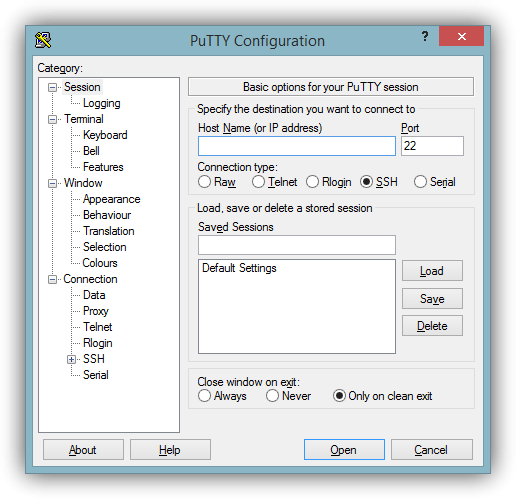
\includegraphics{putty-tutorial-foto-1.png}
    \caption{Pantalla principal de PuTTY}
    \label{putty1}
\end{figure}
\section{Subir y descargar archivos del servidor}
En esta secci\'on se describir\'an algunos m\'etodos que permiten la subida de archivos desde
la m\'aquina local al servidor remoto y la descarga de archivos desde este.
\subsection{SFTP (SSH File Transfer Protocol)}
Es un protocolo de red que permite la transferencia de archivos entre dos m\'aquinas. A continuaci\'on, se describir\'a el uso de este protocolo mediante la l\'inea de comandos y desde FileZilla.
\subsubsection{Desde la l\'inea de comandos}
Para conectar v\'ia SFTP a un servidor remoto, escribir el siguiente comando:
\begin{verbatim}
      my_username@host:$ sftp username@host_ip_address
\end{verbatim}
Nos pedir\'a ingresar la contrase\~na del usuario con el cual queremos acceder y
una vez ingresada y validada estaremos en el prompt de SFTP.
Para subir un archivo escribimos:
\begin{verbatim}
      sftp> put local_file
\end{verbatim}
Una vez ejecutado devolver\'a la ruta del servidor donde fue guardado el archivo.\\
Para subir una carpeta tambien ejecutamos put pero debemos primero crear la carpeta en el servidor ejecutando el comando mkdir, despu\'es, ejecutamos put con el parametro -r el cual se encarga de que los subdirectorios y sus archivos tambien sean subidos como se muestra a continuaci\'on:
\begin{verbatim}
      sftp> mkdir local_folder
      sftp> put -r local_folder
\end{verbatim}
Es importante aclarar que el nombre de la carpeta creada 
en el servidor y el nombre de la carpeta a subir deben coincidir.\\
Para descargar archivos desde el servidor debemos conectarnos v\'ia 
SFTP como se muestra en y ejecutar:
\begin{verbatim}
      sftp> get remote_file
\end{verbatim}
Esto descargara el archivo llamado remote\_file y asi mismo sera guardado en local.
Si queremos guardar el archivo descargado con otro nombre, podemos agregar un segundo parametro como se muestra a continuacion:
\begin{verbatim}
      sftp> get remote_file local_file
\end{verbatim}
Si lo que queremos descargar es un directorio, podemos agregar el par\'ametro -r antes de el nombre de este:
\begin{verbatim}
      sftp> get -r remote_directory
\end{verbatim}
Otro par\'ametro \'util al descargar archivos es -P, us\'andolo, podemos descargar el archivo o el directorio con los mismos permisos que se ten\'ia en el servidor:
\begin{verbatim}
      sftp> get -P remote_file
\end{verbatim}
\end{document}